\documentclass{assignment}
\usepackage{enumitem}
\usepackage{graphicx}
\usepackage{tabularray}
\usepackage{etoolbox}

\BeforeBeginEnvironment{tblr}{
\begin{center}}
    \AfterEndEnvironment{tblr}{
\end{center}}

\SetTblrInner{
    colsep = 4pt,
    cells = {font = \small},
    row{1} = {
        font = \small\bfseries,
        bg = gray!15,
        valign = m
    },
    hline{2} = {1.2pt}
}

\begin{document}
\assignmentTitle{Pham Xuan Hoang}{2640009}{assets/usth_logo.png}%
{Information Systems}{Labwork 5}

\section*{\texttt{employee} table}
\begin{figure}[h]
    \centering
    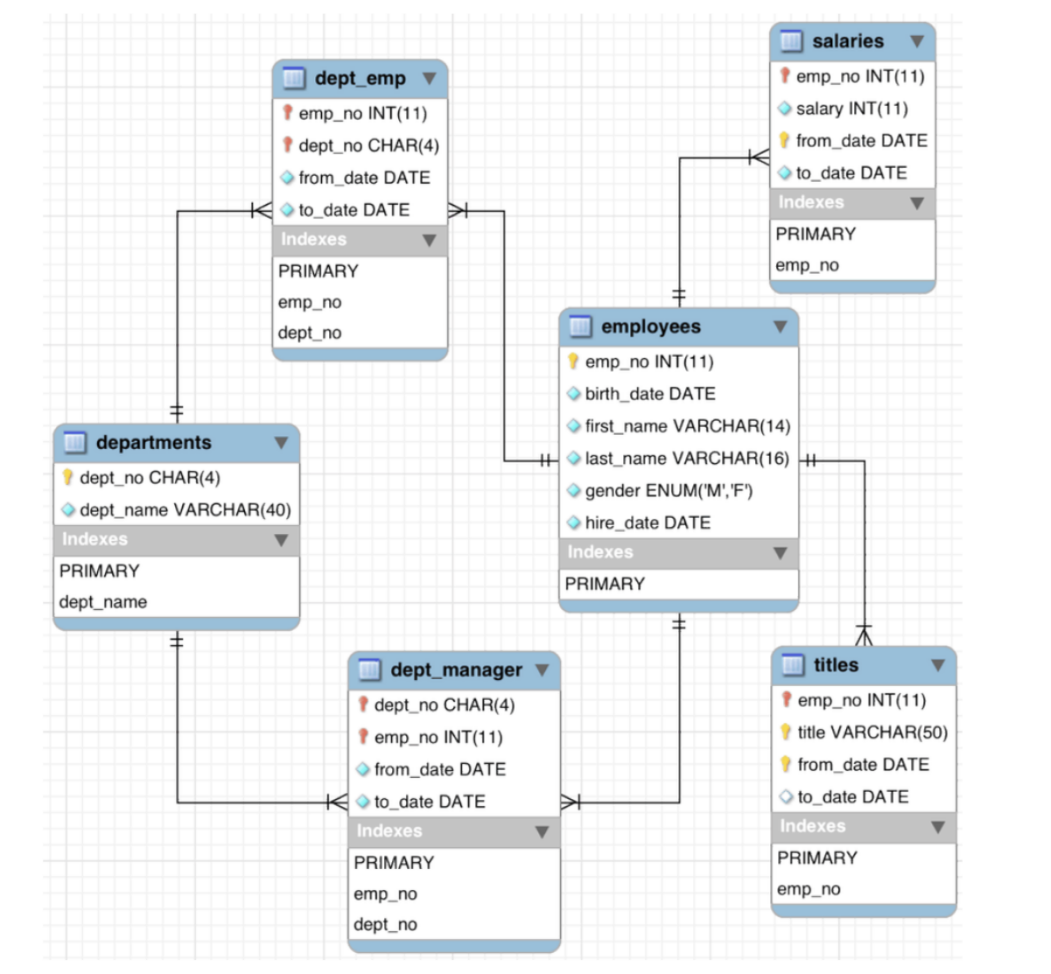
\includegraphics[width=0.7\linewidth]{assets/employees_schema.png}
    \caption{\texttt{employees} database schema}
\end{figure}

\paragraph{1NF.} Every column holds a single atomic value (no lists, no
comma-separated values), and no table has repeated columns. In
particular, histories are stored as \emph{rows}, not as columns: an
employee's salaries are many rows of \texttt{salaries}, not columns
\texttt{salary1}, \texttt{salary2}, \ldots{} Every table has a primary
key, so no two rows are identical.

\paragraph{2NF.} A partial dependency is only possible when the primary
key is composite, so:
\begin{itemize}[noitemsep]
    \item \texttt{employees} (key \texttt{emp\_no}) and
        \texttt{departments} (key \texttt{dept\_no}) have single-column
        keys and are in 2NF automatically.
    \item \texttt{dept\_emp} and \texttt{dept\_manager} each have one
        composite primary key (\texttt{emp\_no}, \texttt{dept\_no}),
        both columns also being foreign keys. \texttt{from\_date} and
        \texttt{to\_date} need the whole key: \texttt{emp\_no} alone is
        not enough (an employee who moved has a different period in each
        department), and neither is \texttt{dept\_no} (a department has
        many employees with different periods).
    \item \texttt{titles} has the composite key (\texttt{emp\_no},
        \texttt{title}, \texttt{from\_date}). \texttt{to\_date} needs all
        three: one employee holds several titles, one title is held by
        many employees, and \texttt{from\_date} distinguishes two
        separate periods with the same title.
    \item \texttt{salaries} has the composite key (\texttt{emp\_no},
        \texttt{from\_date}). \texttt{salary} and \texttt{to\_date} need
        both: \texttt{emp\_no} alone is not enough (an employee gets a
        new salary every year), and neither is \texttt{from\_date}
        (many employees get a raise on the same day with different
        amounts).
\end{itemize}

\paragraph{3NF.} No non-key column determines another non-key column:
\begin{itemize}[noitemsep]
    \item \texttt{employees}: none of \texttt{birth\_date},
        \texttt{first\_name}, \texttt{last\_name}, \texttt{gender},
        \texttt{hire\_date} determines another. For example,
        \texttt{first\_name} $\not\rightarrow$ \texttt{gender}: two
        employees can share a first name and have different genders.
    \item \texttt{departments}: the only non-key column,
        \texttt{dept\_name}, is \texttt{UNIQUE}, so it is a second
        candidate key, not a transitive dependency.
    \item \texttt{dept\_emp}, \texttt{dept\_manager}: between
        \texttt{from\_date} and \texttt{to\_date}, neither determines
        the other (the length of a period varies).
    \item \texttt{titles} has a single non-key column (\texttt{to\_date}),
        so it cannot have a transitive dependency.
    \item \texttt{salaries}: \texttt{salary} $\not\rightarrow$
        \texttt{to\_date} and \texttt{to\_date} $\not\rightarrow$
        \texttt{salary}; the same amount can be paid over different
        periods.
\end{itemize}

\begin{tblr}{colspec={|l|l|l|l|l|}, hlines}
    Table & PK & {1NF: Columns with\\atomic value, no list\\in column}
    & {2NF: Is there any
    \\ composite key?} & {3NF: Are there any \\ non-key $\rightarrow$
    non-key?} \\

    \texttt{employees} & \underline{\texttt{emp\_no}}
    & {\texttt{birth\_date}, \texttt{first\_name}, \\
    \texttt{last\_name}, \texttt{gender},\\\texttt{hire\_date}} &
    None, only \underline{\texttt{emp\_no}} & {None, all attributes
    \\ depend on \underline{\texttt{emp\_no}}} \\

    \texttt{departments} & \underline{\texttt{dept\_no}} &
    \texttt{dept\_name} & None, only \underline{\texttt{dept\_no}} &
    {None, only one attribute\\ and one primary key}\\

    \texttt{dept\_emp} &
    {\underline{\texttt{emp\_no}}\\\underline{\texttt{dept\_no}}}
    & \texttt{from\_date}, \texttt{to\_date} & {1 composite
        PK \underline{\texttt{dept\_no}} \\and
        \underline{\texttt{emp\_no}}, both
    are\\ primary keys and both\\are foreign keys too} & {None,
    \texttt{from\_date} and\\ \texttt{to\_date} are independent} \\

    \texttt{dept\_manager} &
    {\underline{\texttt{emp\_no}}\\\underline{\texttt{dept\_no}}}
    & \texttt{from\_date}, \texttt{to\_date} & Same as \texttt{dept\_emp} &
    Same as \texttt{dept\_emp}\\

    \texttt{titles} &
    {\underline{\texttt{emp\_no}}
        \\ \underline{\texttt{title}}
    \\ \underline{\texttt{from\_date}}} & \texttt{to\_date} & {1
        composite PK \underline{\texttt{emp\_no}},\\
        \underline{\texttt{title}} and
        \underline{\texttt{from\_date}}\\with
    \underline{\texttt{emp\_no}} is also a\\foreign key} & {None,
    \texttt{to\_date} depends\\on the entire composite key} \\

    \texttt{salaries} & {\underline{\texttt{emp\_no}}
    \\ \underline{\texttt{from\_date}}} & {\texttt{salary},
    \texttt{to\_date}} & {1 composite key of\\
        \underline{\texttt{emp\_no}} and \underline{\texttt{from\_date}}\\
    with \underline{\texttt{emp\_no}} is also a\\foreign key} & {None,
    \texttt{salary} and \texttt{to\_date}\\requires the entire composite\\key}\\
\end{tblr}

The \texttt{employee} database satisfies third normal form (3NF).
\begin{enumerate}[noitemsep]
    \item In all tables, each column contains atomic value and there
        are no repeated columns within a table
        $\rightarrow$ \texttt{employee} satisfies first normal form (1NF)
    \item All non-key column depends on the primary keys:
        \begin{itemize}
            \item \texttt{employees} table: all attributes are
                identified by the primary key \texttt{emp\_no}.
            \item \texttt{titles} table: this table has a composite
                primary key. It consists of \texttt{emp\_no},
                \texttt{title} and \texttt{from\_date}. Of which,
                \texttt{emp\_no} is also a foreign key linking
                \texttt{titles} to \texttt{employees}.
            \item \texttt{departments} table: this table contains a
                primary key of \texttt{dept\_no} and attribute
                \texttt{dept\_name} which is unique and depends on the
                primary key.
            \item \texttt{dept\_emp} and \texttt{dept\_manager} both
                have two primary key which happen to be foreign key.
                \texttt{emp\_no} links back to table
                \texttt{employees} and \texttt{dept\_no} links back to
                \texttt{departments}.
        \end{itemize}
    \item It has no transitive dependencies, all the non-key columns
        depends on the key column.
\end{enumerate}

\section*{Order form}
Normalize the following document to 3NF
\begin{center}
    \begin{tabular}{|l|l|c|c|}
        \hline
        \multicolumn{4}{|c|}{Order Form} \\ \hline
        \multicolumn{1}{|l}{Order number} & \multicolumn{3}{l|}{on7126} \\
        \multicolumn{1}{|l}{Order date} & \multicolumn{3}{l|}{11/07/2016} \\
        \multicolumn{1}{|l}{Customer name} & \multicolumn{3}{l|}{Tran
        Giang Son} \\
        \multicolumn{1}{|l}{Customer phone} & \multicolumn{3}{l|}{+84-4
        37 91 69 60} \\
        \multicolumn{1}{|l}{Customer address} & \multicolumn{3}{l|}{18
        Hoang Quoc Viet} \\
        \multicolumn{1}{|l}{City} & \multicolumn{3}{l|}{Hanoi,
        Vietnam} \\ \hline
        ProdId & Description & Quantity & Price \\ \hline
        P101 & Intel i7 6700K & 1 & \$349 \\ \hline
        P102 & ASUS Z170A-P & 1 & \$149 \\ \hline
        P103 & Corsair DDR4 4 $\times$ 8GB & 1 & \$469 \\ \hline
        P104 & Samsung EVO 850 512GB & 1 & \$249 \\ \hline
        P105 & GeForce GTX 1080 8G & 1 & \$725 \\ \hline
        P106 & Corsair CS750M 80+ Gold & 1 & \$119 \\ \hline
        P107 & Corsair Carbide 400R Mid & 1 & \$85 \\ \hline
    \end{tabular}
\end{center}

\noindent Order database schema normalized to 3NF

\begin{figure}[h]
    \centering
    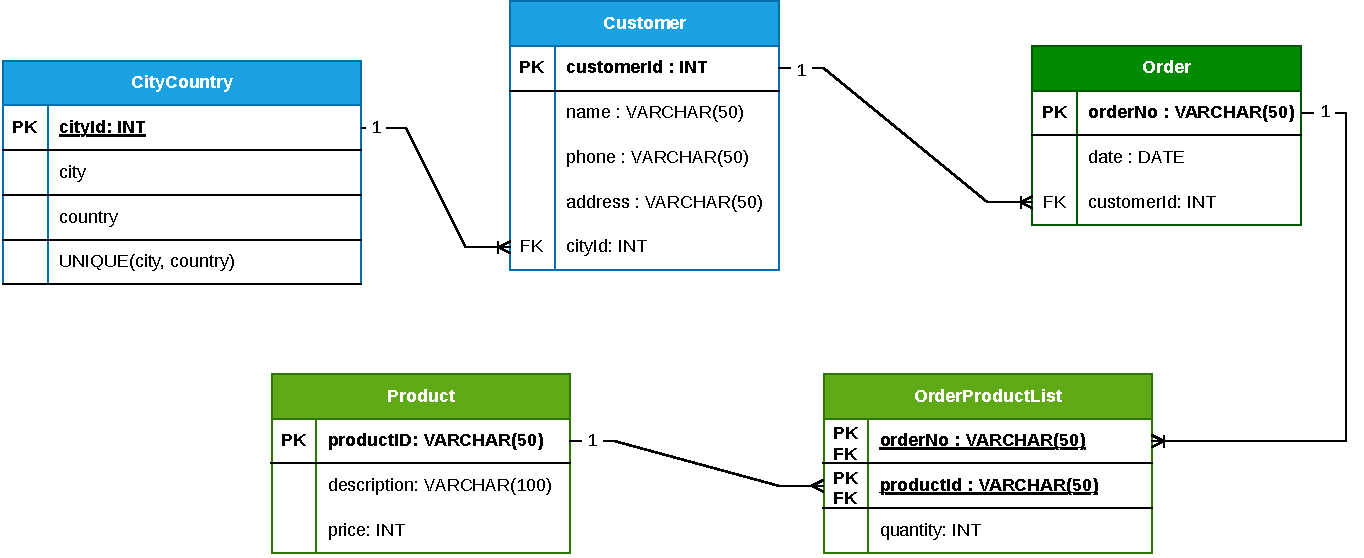
\includegraphics[width=0.7\linewidth]{assets/computer_order.pdf}
    \caption{Order database schema}
\end{figure}

\end{document}
